\documentclass[11pt]{article}
\usepackage[letterpaper,margin=1in]{geometry}
\usepackage{amsmath,amssymb,amsthm}
\usepackage{graphicx}
\usepackage{booktabs}
\usepackage{caption}
\usepackage{subcaption}
\usepackage{enumitem}
\usepackage{titlesec}
\usepackage{fancyhdr}
\usepackage{placeins}
\usepackage{float}
\usepackage{xcolor}
\PassOptionsToPackage{hyphens}{url}
\usepackage[hidelinks]{hyperref}
\usepackage{xurl}
\setlength{\parskip}{0.4em}
\setlength{\parindent}{0pt}
\setlength{\emergencystretch}{2em}
\titleformat{\section}{\large\bfseries}{\thesection.}{0.6em}{}
\titlespacing*{\section}{0pt}{1.4em}{0.5em}
\titleformat{\subsection}{\normalsize\bfseries}{\thesubsection}{0.5em}{}
\titlespacing*{\subsection}{0pt}{1.0em}{0.3em}
\captionsetup{font=small,labelfont=bf,labelsep=period,skip=6pt}
\setlist[itemize]{leftmargin=1.3em,itemsep=2pt,topsep=3pt,parsep=0pt}
\setlist[enumerate]{leftmargin=1.6em,itemsep=2pt,topsep=3pt,parsep=0pt}
\pagestyle{fancy}
\fancyhf{}
\fancyhead[L]{\small CS 6362: Advanced Machine Learning}
\fancyhead[R]{\small Assignment 2 \,\textbar\, Bibek Dhungana}
\fancyfoot[C]{\small\thepage}
\renewcommand{\headrulewidth}{0.4pt}
\newcommand{\code}[1]{\texttt{#1}}
\newcommand{\repo}[1]{\nolinkurl{#1}}   % repository names, may break at / and -
\newcommand{\E}{\mathbb{E}}
\newcommand{\R}{\mathbb{R}}
\newcommand{\KL}[2]{D_{\mathrm{KL}}\!\left(#1\,\|\,#2\right)}
\newcommand{\TODO}[1]{\textcolor{red}{[#1]}}
\newtheorem{theorem}{Theorem}

\begin{document}
\begin{center}
  {\LARGE\bfseries Paper 3: $\beta$-VAE: Learning Basic Visual Concepts\\[2pt] with a Constrained Variational Framework}\\[5pt]
  {\large Higgins, Matthey, Pal, Burgess, Glorot, Botvinick, Mohamed, Lerchner (ICLR 2017)}\\[4pt]
  Bibek Dhungana \quad\textbar\quad CS 6362 Assignment 2 \quad\textbar\quad \today
\end{center}

\section{Problem statement and summary}

\subsection{Setup}
The data are binary images $x\in\{0,1\}^{64\times64}$ of one white shape on a black background (the dSprites or ``2D shapes'' dataset). Each image is generated from five factors $v=(\text{shape},\text{scale},\text{rotation},\text{position }X,\text{position }Y)$ with $3\times6\times40\times32\times32=737{,}280$ combinations. Every combination appears exactly once, so the factors are independent, and $x=\mathrm{Sim}(v)$ has no other randomness.

The goal is to learn, without ever seeing $v$, an encoder that maps an image to a code $z\in\R^{10}$ that is \emph{disentangled}: each coordinate $z_j$ that carries information should react to one factor and ignore the others. Figure~7 of the paper checks this by plotting how each coordinate responds to each factor.

\subsection{From the VAE to the \texorpdfstring{$\beta$}{beta}-VAE}
The model has a prior $p(z)=\mathcal N(0,I)$, a decoder $p_\theta(x\mid z)$ that gives every pixel a Bernoulli probability, and an encoder $q_\phi(z\mid x)=\mathcal N\big(\mu_\phi(x),\operatorname{diag}\sigma^2_\phi(x)\big)$. Since $\log p_\theta(x)$ is generally intractable to compute exactly, the VAE maximizes a lower bound on it, which follows from writing $p_\theta(x)=\E_{q_\phi}\big[p_\theta(x\mid z)\,p(z)/q_\phi(z\mid x)\big]$ and applying Jensen's inequality:
\[
  \log p_\theta(x)\ \ge\ \underbrace{\E_{q_\phi(z\mid x)}[\log p_\theta(x\mid z)]}_{\text{reconstruction}}-\underbrace{\KL{q_\phi(z\mid x)}{p(z)}}_{\text{cost of the code}}=\text{ELBO}.
\]
The paper starts instead from a constrained problem: reconstruct as well as possible while keeping the code close to the prior,
\[
  \max_{\theta,\phi}\ \E_{q_\phi(z\mid x)}[\log p_\theta(x\mid z)]\quad\text{subject to}\quad \KL{q_\phi(z\mid x)}{p(z)}<\epsilon .
\]
With a Lagrange multiplier $\beta\ge0$ this becomes $\E_q[\log p_\theta(x\mid z)]-\beta\,(\mathrm{KL}-\epsilon)$, and dropping the constant $\beta\epsilon$ gives the $\beta$-VAE objective
\[
  \mathcal L_\beta(\theta,\phi;x)=\E_{q_\phi(z\mid x)}[\log p_\theta(x\mid z)]-\beta\,\KL{q_\phi(z\mid x)}{p(z)} .
\]
$\beta=1$ is the ordinary VAE.

For a Gaussian encoder the KL of one latent with mean $\mu$ and variance $\sigma^2$ is $\tfrac12(\mu^2+\sigma^2-1-\log\sigma^2)$, which follows from $\E_q(z-\mu)^2=\sigma^2$ and $\E_q z^2=\mu^2+\sigma^2$. An unused latent ($\mu=0$, $\sigma^2=1$) costs nothing, while a latent with $\sigma^2=0.01$ and $\mu^2\approx1$ costs about 2.3 nats. Small learned variance is a useful activity heuristic. A variance near 1 means a latent is unused only when its mean is also near zero and independent of the input.

For dSprites, Table~1 of the paper gives a fully connected model: encoder $4096\to1200\to1200\to$ 10 means and 10 log-variances with ReLU, decoder $10\to1200\to1200\to1200\to4096$ with tanh and Bernoulli outputs, trained with Adagrad at learning rate $10^{-2}$. The VAE baseline is the same model with $\beta=1$.

\subsection{Answers to the questions in the assignment}
\textbf{What happens to $\mathcal L_\beta$ for $\beta>1$ and for $\beta<1$?} Write $\mathcal L_\beta=\text{ELBO}-(\beta-1)\,\mathrm{KL}$. For $\beta>1$ we subtract something non-negative, so $\mathcal L_\beta\le\text{ELBO}\le\log p_\theta(x)$: still a lower bound on the log-likelihood, but a looser one, and maximizing it gives up some reconstruction to keep the code closer to the prior. I think of the KL as the number of nats the code spends on an image and of $\beta$ as the price per nat: when nats are expensive, the model only buys what helps reconstruction most (where the shape is, then how big it is) and switches the other latents off. The paper argues that this pressure also pushes each factor into its own latent, because the prior treats the latents as independent and each one pays its own KL. For $\beta<1$ the penalty is weaker and $\mathcal L_\beta\ge\text{ELBO}$, so it is no longer guaranteed to be below $\log p_\theta(x)$. The weaker penalty permits more information in the code, but does not require the factors to mix. At $\beta=0$ only expected reconstruction remains; the encoder is still stochastic unless its variance collapses or sampling is removed.

\textbf{How are the latents in Figure 7 ordered, and how is each traversal generated?} Each column is one latent $z_i$, and the columns are sorted by learned variance (the average of $\sigma_i^2(x)$ over the data), smallest first. So the most informative latent comes first and unused latents come last. Rows 1 to 3 show the average of $\mu_i(x)$ as a function of one factor: a $32\times32$ map over position, and curves against scale and rotation with one curve per shape (square red, oval green, heart blue). For the traversals, one image is encoded, nine latents are kept at their inferred means, the remaining one is set to values from $-3$ to $3$ (three prior standard deviations), and the decoder output is shown.

\section{Reproduction of Figure 7A and 7B}

\subsection{LLM, conversation and code}
\begin{itemize}
  \item \textbf{LLM:} ChatGPT (GPT-5.6) for the main conversation. I also asked Claude and Gemini some side questions to understand concepts related to the paper.
  \item \textbf{Shared conversation}:\newline \url{https://chatgpt.com/share/e/6ad7087d-51d0-83e9-8f59-be137ca3d921}
  \item \textbf{Code:} folder \code{paper3: beta-VAE/code} of\newline \url{https://github.com/dhunganabibek/reading-and-reproducing-papers}. The notebook \code{reproduce\_fig7.ipynb} displays the saved figures and measurements by default. It can train the models and regenerate the figures; large weights are excluded from Git.
\end{itemize}

\subsection{Setup and choices}
\begin{table}[H]\centering\small
  \begin{tabular}{@{}l@{\quad}p{0.76\textwidth}@{}}
    \toprule
    Data & dSprites, all 737{,}280 images, no train/test split\\
    Model & fully connected encoder and decoder of the paper's Table~1, 10 latents, Bernoulli likelihood\\
    Objective & $-\mathcal L_\beta$ with $\beta=1$ and $\beta=4$; one extra model with $\beta=16$\\
    Optimizer & Adagrad, learning rate $10^{-2}$ (paper), accumulator started at 0.1; batch 256, 30 epochs, i.e.\ 86{,}400 updates (my choices)\\
    Seeds & 3 per $\beta$ for $\beta=1$ and $\beta=4$; for a given seed both $\beta$ start from the same weights\\
    Figure & latents sorted by learned variance; five most informative and one unused; traversal values $3,\,1.5,\,0,\,-1.5,\,-3$\\
    \bottomrule
  \end{tabular}
  \caption{Setup of my runs.}
\end{table}

\textbf{How many seeds, and what one seed can and cannot show.} I trained three seeds per $\beta$. One seed can show that the difference in Figure~7 \emph{can} happen with this model, but not that it happens \emph{reliably}, because it cannot tell a typical result from a lucky one. My runs show this (Table~\ref{tab:seeds}): with seed 0 alone I would report a large effect of $\beta$, with seed 1 alone almost none. The paper used ten seeds per model for its score and discarded the worse half (Appendix~A.4), and it does not say how the model in Figure~7 was picked. I show seed 0 because it is the first seed, not because it is the best. Models in each training group share minibatch order, so these are comparisons across initializations with paired data order, not independent replications of all training randomness.

\begin{figure}[t]\centering
  \begin{minipage}[b]{0.51\textwidth}\centering
    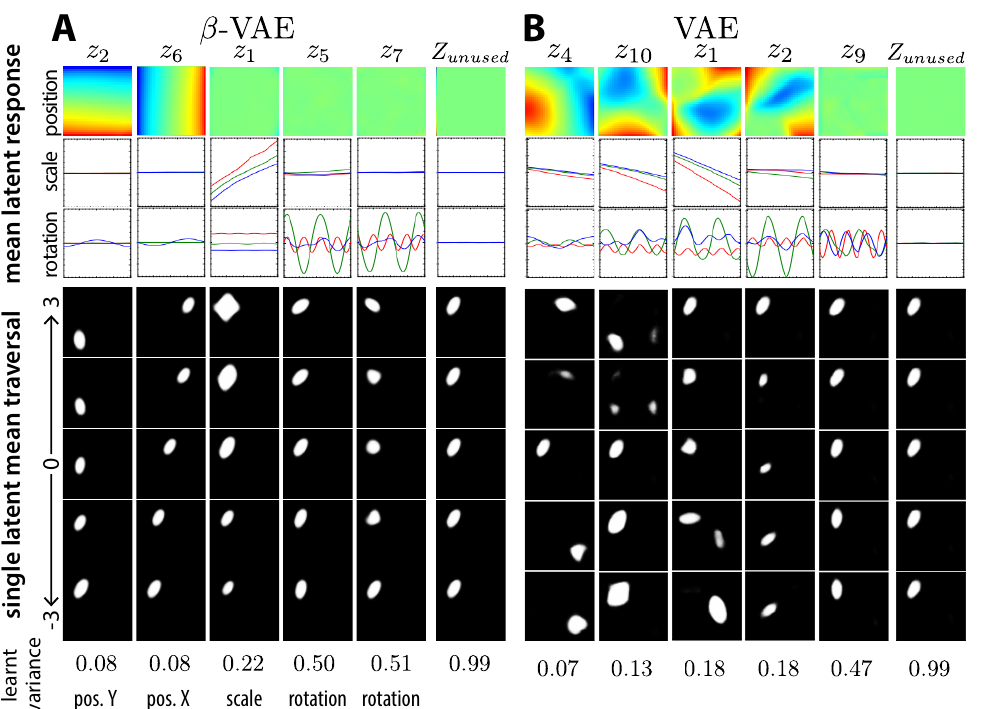
\includegraphics[width=\linewidth]{figures/original_fig7ab.png}\\[2pt]
    {\small (a) the paper}
  \end{minipage}\hfill
  \begin{minipage}[b]{0.46\textwidth}\centering
    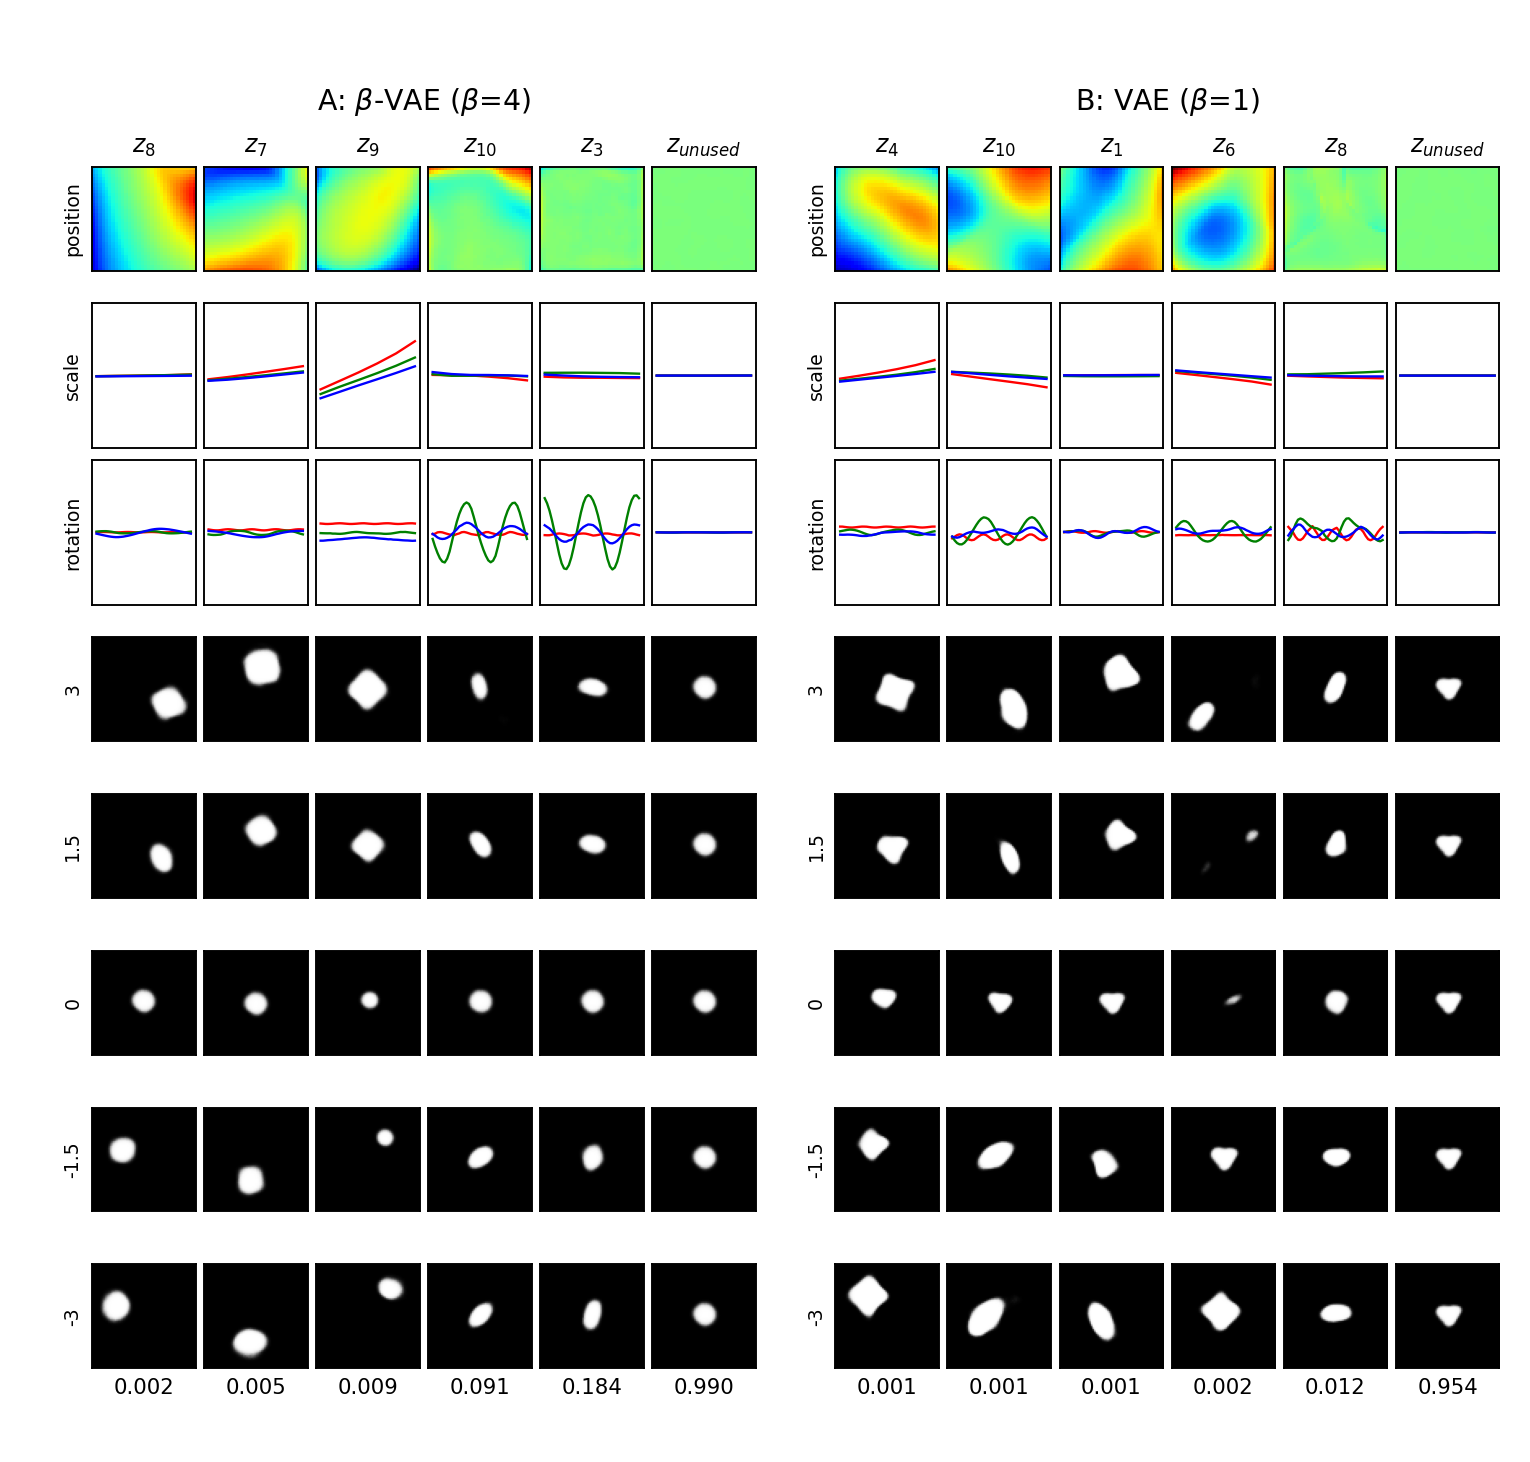
\includegraphics[width=\linewidth]{figures/fig7ab_reproduced.png}\\[2pt]
    {\small (b) my reproduction, seed 0}
  \end{minipage}
  \caption{Figure 7A ($\beta$-VAE, $\beta=4$) and 7B (VAE). Rows 1--3: mean response of each latent to position, scale and rotation (one curve per shape). Rows 4--8: decoder output when the latent is moved from $3$ to $-3$. The number below each column is the learned variance.}
  \label{fig:fig7}
\end{figure}

\subsection{Results}
\textbf{What Figure 7 is evidence for.} A disentangled latent has a mean that changes with one factor and stays flat for the others, and moving it changes one property of the image. In the paper's panel A ($\beta=4$) this holds for five latents: vertical position, horizontal position, scale, and two for rotation. In panel B (the VAE) the position maps are blobs, several rows react in the same column, and a traversal changes several things at once.

\textbf{My figure shows the same difference.} For $\beta=4$ the first two latents have position maps close to planes, one mostly horizontal and one mostly vertical, with flat scale and rotation curves. The third reacts mainly to scale, the fourth and fifth mainly to rotation, and five latents are unused. For $\beta=1$ four latents react to position, but none along one image axis, and their traversals change position, size and outline together. Table~\ref{tab:latents} puts numbers on rows 1 to 3: for every used latent, the fraction of the variance of its mean that one factor explains on its own.

\begin{table}[H]\centering\small
  \begin{tabular}{@{}l l cc ccccc c@{}}
    \toprule
    & & learned & KL & \multicolumn{5}{c}{fraction of variance explained by} & $X$ and $Y$\\
    \cmidrule(lr){5-9}
    model & latent & variance & (nats) & shape & scale & rotation & $X$ & $Y$ & together\\
    \midrule
    $\beta=4$ & $z_8$ & 0.002 & 3.28 & 0.00 & 0.00 & 0.00 & \textbf{0.82} & 0.13 & 0.96\\
    & $z_7$ & 0.005 & 2.99 & 0.00 & 0.02 & 0.00 & 0.06 & \textbf{0.69} & 0.86\\
    & $z_9$ & 0.009 & 2.44 & 0.07 & \textbf{0.30} & 0.00 & 0.18 & 0.18 & 0.53\\
    & $z_{10}$ & 0.091 & 1.43 & 0.00 & 0.00 & \textbf{0.28} & 0.01 & 0.13 & 0.26\\
    & $z_3$ & 0.184 & 0.92 & 0.01 & 0.00 & \textbf{0.50} & 0.00 & 0.00 & 0.01\\
    \addlinespace
    $\beta=1$ & $z_4$ & 0.001 & 3.67 & 0.01 & 0.03 & 0.00 & 0.30 & \textbf{0.38} & 0.85\\
    & $z_{10}$ & 0.001 & 3.48 & 0.01 & 0.01 & 0.05 & 0.11 & \textbf{0.18} & 0.77\\
    & $z_1$ & 0.001 & 3.52 & 0.00 & 0.00 & 0.01 & \textbf{0.39} & 0.27 & 0.82\\
    & $z_6$ & 0.002 & 3.38 & 0.01 & 0.02 & 0.03 & \textbf{0.35} & 0.34 & 0.79\\
    & $z_8$ & 0.012 & 2.31 & 0.00 & 0.00 & \textbf{0.05} & 0.00 & 0.00 & 0.02\\
    \bottomrule
  \end{tabular}
  \caption{What each used latent encodes (seed 0). ``Rotation'' is rotation within a shape. The largest single-factor entry of each latent is in bold.}
  \label{tab:latents}
\end{table}

With $\beta=4$ one latent is explained 82\% by $X$ alone and another 69\% by $Y$ alone. With $\beta=1$ no latent gets above 39\% from one factor, and each position latent needs $X$ and $Y$ together (0.77 to 0.85). This supports the qualitative comparison for seed 0, though less cleanly than in the paper: my $X$ latent is slightly tilted, the scale latent also moves the shape, and the rotation fractions are low.

The paper says the rotation latents oscillate with each shape's symmetry: once per full turn for the heart, twice for the oval, four times for the square. In my $\beta=4$ model the oval has two periods and the square four, but the heart also has two. My model encodes the direction of a shape's long axis, not which way a heart points, which fits the traversals, where the decoder draws a blob rather than a heart.

\begin{table}[tb]\centering\small
  \begin{tabular}{@{}cc c c cc c@{}}
    \toprule
    & & used & KL & \multicolumn{2}{c}{reconstruction from the code mean} & single-factor\\
    \cmidrule(lr){5-6}
    $\beta$ & seed & latents & (nats) & $-\log p(x\mid z)$ (nats) & wrong pixels & fraction\\
    \midrule
    1 & 0 & 5 & 16.4 & 47.6 & 17.7 & 0.27\\
    1 & 1 & 5 & 16.5 & 44.6 & 16.5 & 0.49\\
    1 & 2 & 5 & 15.3 & 57.5 & 21.8 & 0.64\\
    \addlinespace
    4 & 0 & 5 & 11.1 & 62.9 & 24.8 & 0.52\\
    4 & 1 & 5 & 11.0 & 62.1 & 24.8 & 0.54\\
    4 & 2 & 4 & 9.9 & 78.6 & 34.1 & 0.76\\
    \addlinespace
    16 & 0 & 3 & 5.9 & 108.6 & 46.2 & 0.44\\
    \bottomrule
  \end{tabular}
  \caption{All models. ``Used'' means a learned variance below 0.5. ``Wrong pixels'' is the number of the 4096 pixels of an image that differ from the data after rounding the decoder output. ``Single-factor fraction'' is the average of the bold entries of Table~\ref{tab:latents}; it is a descriptive statistic, not the paper's disentanglement score. All measurements use the training grid, so they do not estimate held-out performance.}
  \label{tab:seeds}
\end{table}

\textbf{All seeds.} For each seed the $\beta=4$ model has the higher single-factor fraction (0.52 against 0.27, 0.54 against 0.49, 0.76 against 0.64), so the direction of the claim is reproduced three times out of three. But the seeds differ as much as the two values of $\beta$ do. The VAE of seed 2 (0.64) is cleaner than the $\beta$-VAEs of seeds 0 and 1, and the $\beta$-VAE of seed 2 uses only four latents, finds $X$, $Y$ and scale cleanly (0.91, 0.84, 0.77), and has no rotation latent. So $\beta$ sets the budget, but which factors the model spends it on depends on the random start.

\textbf{Would a larger $\beta$ help further, and what happens to reconstruction?} Not indefinitely. A larger $\beta$ means fewer nats in the code (about 16, 11 and 6 for $\beta=1$, 4, 16) and worse reconstruction (17 to 22 wrong pixels per image at $\beta=1$, 25 to 34 at $\beta=4$, 46 at $\beta=16$). My $\beta=16$ model uses three latents, keeps position and rough size, loses rotation and shape (Figure~\ref{fig:recon}), and is less clean than at $\beta=4$ (single-factor fraction 0.44). At a very high price the model can only afford the most valuable factor, and the others are squeezed together or dropped. The paper reports the same rise and fall of disentanglement with $\beta$ (Section~4.2). For a very large $\beta$ the code carries nothing and the decoder draws the average image.

\begin{figure}[tb]\centering
  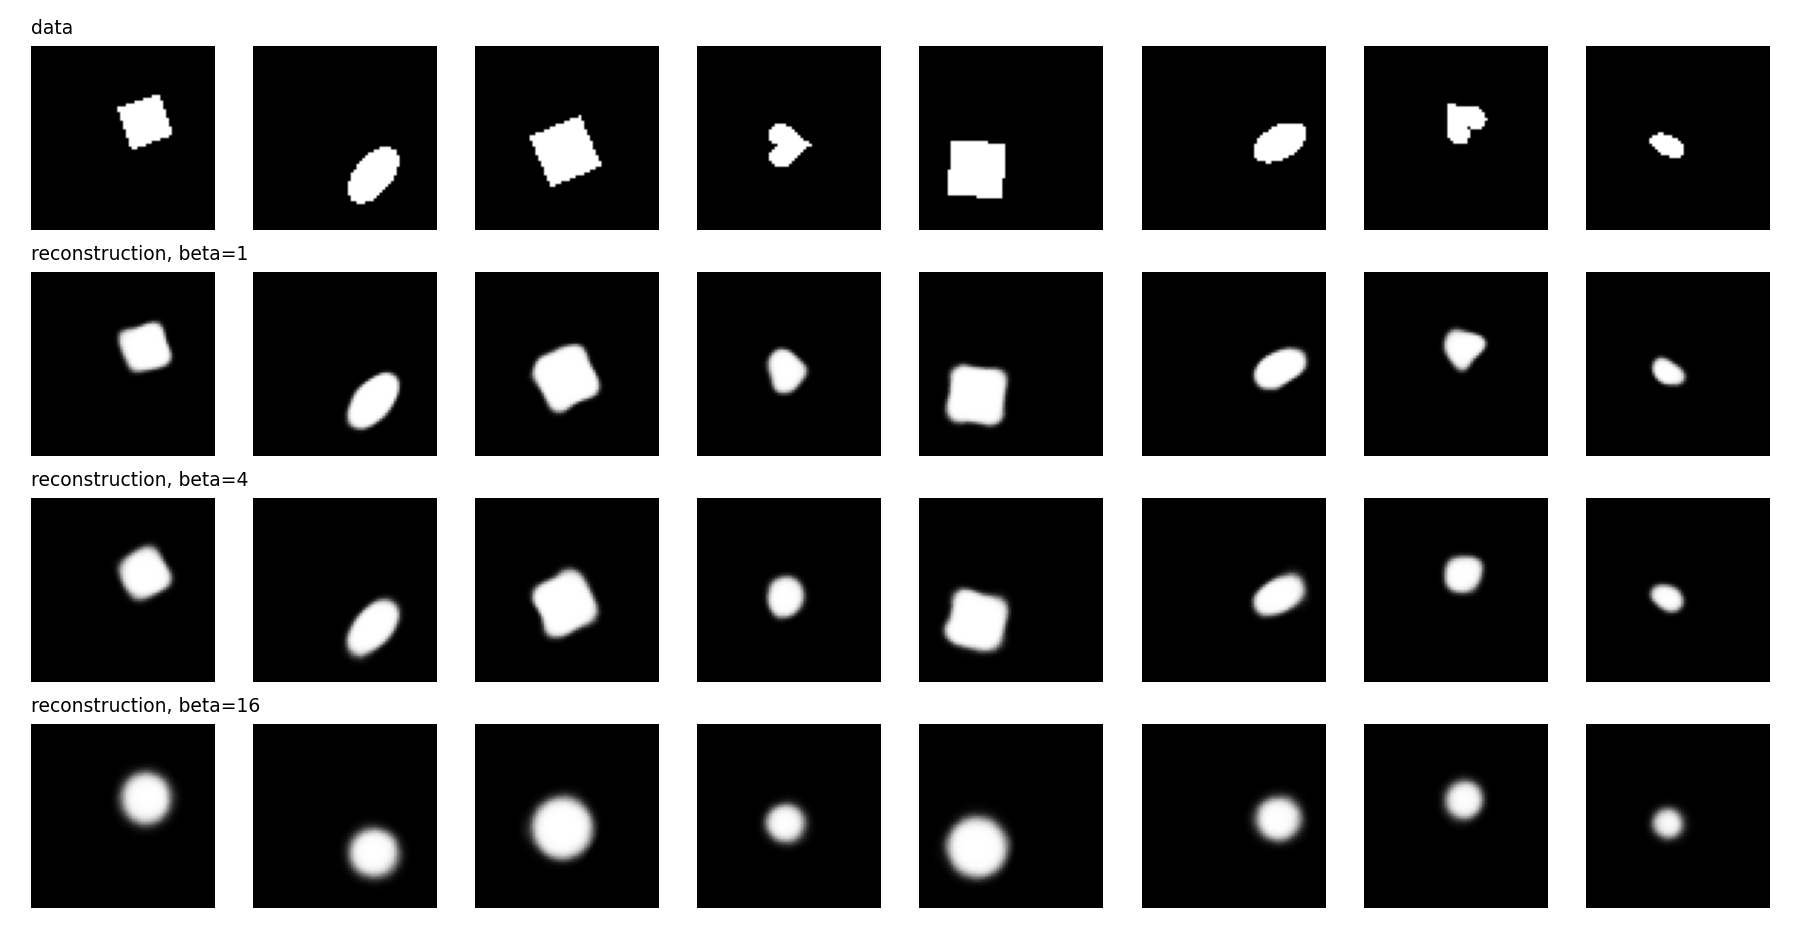
\includegraphics[width=0.66\textwidth]{figures/reconstructions.png}
  \caption{Data and reconstructions from the code mean for $\beta=1$, 4 and 16 (seed 0). At $\beta=4$ the hearts have become blobs; at $\beta=16$ every shape is a round blob of about the right size in the right place.}
  \label{fig:recon}
\end{figure}

\subsection{Phases 1--3: failures and corrections}
In Phase~1 I gave the LLM the paper and asked for a PyTorch reproduction of Figure~7A and 7B. Checking its output against the paper and running the code (Phases 2 and 3) turned up these problems:
\begin{itemize}
  \item \textbf{Wrong architecture.} The first plan used a convolutional VAE, which the paper uses for chairs, faces and celebA. Table~1 gives a fully connected model for the 2D shapes. I caught this before any code was written.
  \item \textbf{Training speed.} With batch size 64, one epoch for two models took about 7 minutes. I switched to batch size 256 and to a trainer that runs several models side by side on the same batches, and checked that one step of it gives exactly the same weights as training each model alone.
  \item \textbf{A violent first step.} When I added $\beta=16$ to the first complete attempt, its KL was $10^{32}$ after one epoch. PyTorch's Adagrad starts with an empty accumulator, so its first update moves each weight with a nonzero gradient by approximately $\pm$ the learning rate, when the gradient magnitude exceeds the numerical epsilon. With 4096 inputs these changes add up, and after one step the largest log-variance in a batch was about 110 instead of 0.09. The $\beta=1$ and $\beta=4$ models recover, but the $\beta=16$ model does not, because Adagrad never forgets the huge gradients that follow. TensorFlow's Adagrad starts the accumulator at 0.1; with that, all three models train, and every result here uses it.
  \item \textbf{A misleading panel.} At first each position map had its own color scale, so an unused latent's map showed noise stretched to the full range and looked structured. All latents of a model now share one color scale, as in the paper.
\end{itemize}

\subsection{What did not match}
\textbf{The learned-variance row.} My used latents have learned variances from 0.002 to 0.18; the paper shows 0.08 to 0.51. The square roots of mine (0.05, 0.07, 0.10, 0.30, 0.43) are close to the paper's row (0.08, 0.08, 0.22, 0.50, 0.51), and the unused latent has 0.99 in both, so the paper's row may show standard deviations. This is a possible explanation, not a verified labeling error. Taking the square root of the reported average variance preserves its order, whereas averaging per-image standard deviations need not.

\textbf{How clean the latents are.} In the paper the position latents follow the image axes exactly and the scale latent is clean. In my seed 0 this is only roughly true; in seed 2 it is true. The paper gives neither the batch size, the training length, nor how its model was chosen from its seeds, so I cannot tell how much of the difference is selection and how much is training.

\subsection{Phase 4}
The authors did not release code for this paper. After saving the Phase~3 code I checked two other sources. The official dSprites repository (\repo{google-deepmind/dsprites-dataset}) confirms the factor order, the shape order (so my curve colors follow the paper), and that every combination appears exactly once. The follow-up paper by the same group (Burgess et al.\ 2018) trains a convolutional model with Adam on dSprites, so it does not settle the open settings of the 2017 paper. One disclosure: while I was looking for the OpenReview reviews, a web search listed the title of a third-party $\beta$-VAE repository. I did not open it.

I changed nothing because of Phase~4. The changes after the Phase~3 snapshot are my own: the batched trainer, the Adagrad accumulator, three seeds and the $\beta=16$ model, the explained-variance table and reconstruction error, and the shared color scale. The final cleanup keeps the saved results, makes the default notebook read committed figures and measurements, and adds a script for the reconstruction comparison. The snapshot already saved the CPU random-number state. New checkpoints also save the active device state; older GPU checkpoints cannot provide exact continuation. Missing weights now produce a clear error when recomputation is requested, rather than silently skipping models.

\section{Critical review}

\subsection{My review}
\textbf{Strengths.} The method is one number with no change to the architecture, so anyone can try it, and it became the standard baseline for this problem. The ``limited budget'' reading explains well why latents get switched off. The dataset, with exact and independent factors, is a lasting contribution, and Figure~7 is a good qualitative test that I could reuse as is.

\textbf{Weaknesses.}
\begin{itemize}
  \item \emph{Why $\beta>1$ should disentangle is argued, not shown.} Independence alone does not identify the intended factors. For independent standard Gaussian factors, $(X+Y)/\sqrt{2}$ and $(X-Y)/\sqrt{2}$ remain independent standard Gaussians. This counterexample does not apply directly to dSprites' discrete uniform positions, and rotating a diagonal Gaussian posterior generally takes it outside the diagonal family. With $\beta=1$ every position latent of my seed 0 is such a mixture, and the outcome changes from seed to seed under the same objective. Locatello et al.\ (2019) later proved that without further assumptions no unsupervised method can pick out the true factors.
  \item \emph{The cost in reconstruction is not reported.} $\mathcal L_\beta$ is not the ELBO for $\beta\ne1$, and no likelihoods or reconstruction errors are given for the models in Figure~7. In my runs $\beta=4$ gets 25 to 34 pixels per image wrong against 17 to 22 at $\beta=1$, and draws a blob where the data has a heart.
  \item \emph{The score is weak.} Kim and Mnih (2018) showed it can give a perfect score to a code in which one factor is not disentangled at all.
  \item \emph{``No a priori knowledge'' is too strong.} $\beta$ is chosen either with the score, which needs the true factors, or by looking at traversals, which needs a person who knows what the factors should be.
\end{itemize}

\textbf{Possible errors and unclear points.}
\begin{itemize}
  \item $\beta$ is called a Lagrange multiplier, but a multiplier is determined by the constraint. Here $\beta$ is set by hand and $\epsilon$ is never used, so the method is a penalty with a tuned weight.
  \item The two rotation latents are presented as a finding (``cos and sin''), but a rotation is a point on a circle, which cannot be mapped continuously onto one real number, so a continuous, injective encoding of the full rotation circle needs at least two real coordinates. The sampled dataset and a lossy encoder need not meet those assumptions, and topology alone does not force the learned coordinates to be sine and cosine.
  \item Batch size and training length are missing for every model in Table~1.
\end{itemize}

\subsection{Comparison with the OpenReview reviews}
\noindent\href{https://openreview.net/forum?id=Sy2fzU9gl}{OpenReview discussion and public reviews}.

The four reviewers gave 7, 5, 7 and 6 and the paper was accepted as a poster. The reviewer who gave 5 made my second point: no log-likelihoods, samples that look worse than InfoGAN's, and no clear reason why this representation is ``better'' than the VAE's. That reviewer also asked how $\beta$ was selected and why one could not just use fewer latents. One reviewer who gave 7 liked the simplicity but found the score close to a correlation measure, and noted that a very large $\beta$ \emph{hurting} disentanglement does not fit the story that a more economical code is more disentangled. The reviewer who gave 6 asked whether the dense sampling of the factors is what makes the method work (Appendix~A.8 of the published paper shows sparser data does hurt) and wanted numbers on real data. The remaining reviewer (7) doubted that interpretable factors can be found without supervision on real data at all.

I agree with the reviewers on the missing likelihoods, the weak score and the selection of $\beta$. My additional concerns are identifiability and the geometric interpretation of the rotation latents.

\end{document}
